\section{Zielsetzung}
\label{sec:Zielsetzung}
In diesem Versuch soll der Lande-Faktor $g_i$, die Aufspaltung $\Delta E$ der
Zeeman-Linien, sowie die Dispersionsgebiete und Auflösevermögen der
Lummer-Gehrcke-Platte bei den Wellenlängen $\lambda = \SI{643.8}{\nano\meter}$
und $\lambda = \SI{480.0}{\nano\meter}$.

\section{Theorie}
\label{sec:Theorie}
\subsection{Berechnung der magnetischen Momente}
\label{sec:Berechnung_magnetischer_Momente}
Die Hüllenelektronen besitzen zwei Drehimpulse, den Bahndrehimpuls ($\vec{l}$)
und den
Spin ($\vec{s}$) mit ihren Quantenzahlen
\begin{align}
  \mid\vec{l}\mid &= \sqrt{l\left(l+1\right)}\hbar \\
  \mid\vec{s}\mid &= \sqrt{s\left(s+1\right)}\hbar
  \label{eqn:Quantenzahlen}
\end{align}
Das magnetische Moment der Drehimpulseinheit \hbar
\begin{align}
  \mu_\text{B} := \frac{1}{2}\text{e}_0 \frac{\hbar}{m_0}
  \label{eqn:bohr}
\end{align}
wird als Bohrsches Magneton bezeichnet. Daraus lassen sich die magnetischen
Momente der Drehimpulse ableiten zu
\begin{align}
  \vec{\mu}_l &= -\mu_\text{B} \frac{\vec{l}}{\hbar} = -\mu_\text{B} \sqrt{l\left(l+1 \right)} \vec{l}_\text{e}\\
  \vec{\mu}_s &= -\text{g}_\text{S} \cdot \frac{\mu_\text{B}}{\hbar} \vec{s} = -\text{g}_\text{S} \mu_\text{B}\sqrt{s\left(s+1 \right)} \vec{s}_\text{e}.
  \label{eqn:momente}
\end{align}
Dabei sind $\vec{l}_\text{e}$ und $\vec{s}_\text{e}$ Einheitsvektoren in die Richtung
des jeweiligen Drehimpulses.
Der Lande-Faktor g$_\text{S}$ eines Elektrons hat dabei den Wert 2. Daraus resultiert die
magnetomechanische Anomalie des Elektrons. Dabei ist das magnetische Moment des
Spins ($s = \sfrac{\num{1}}{\num{2}}$) doppelt so groß wie für den Bahndrehimpuls
($l = \num{1}$).

\subsection{Wechselwirkung magnetischer Momente und Drehimpulse}
\label{sec:Wechselwirkungen}
Die Drehimpulse der Elektronen in einem Atom können auf verschiedene Arten
miteinander wechselwirken. Hier unterscheiden wir die Grenzfälle bei Atomen mit
niedriger und hoher Kernladungszahl.

Werden die Atome mit niedriger Kernladungszahl betrachtet, so können die Bahndrehimpulse
der Elektronen in den nicht abgeschlossenen Schalen vektoriell aneinander koppeln.
Den daraus entstehenden Impuls nennt man Gesamtdrehimpuls der Hülle
\begin{align}
  \vec{L} = \sum_i \vec{l}_i
  \label{eqn:gesamtbahndrehimpuls}
\end{align}
mit dem Betrag
\begin{align}
  \mid\vec{L}\mid = \sqrt{L\left(L+1 \right)} \hbar.
  \label{eqn:betraggesamtdrehipuls}
\end{align}
Der Gesamtdrehimpuls ist immer ganzzahlig, obwohl die einzelnen Bahndrehimpulse $\vec{l}_i$,
wie in Abbildung \ref{abb:drehimpulse} zu sehen, unterschiedlich koppeln können.
Je nach Gesamtdrehimpulsquantenzahl der Hülle L werden die Terme mit S, D, P und F
unterschieden (Drehimpulsdrehsymbole).
\begin{figure}[htb]
  \centering
  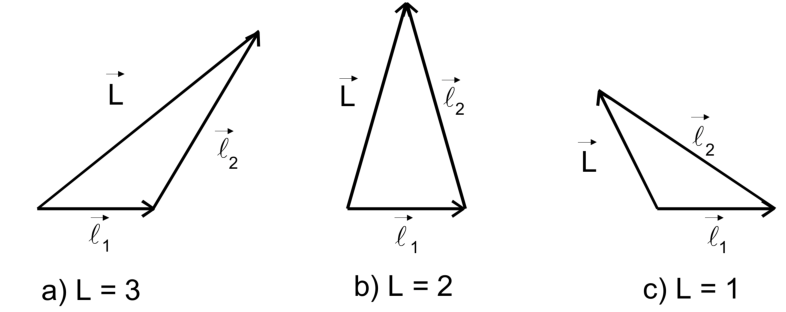
\includegraphics[width=0.8\textwidth]{images/V27.pdf}
  \caption{Vektorielle Kombination von zwei Drehimpulsen zu einem Gesamtdrehimpuls
  \cite{anleitung}. Hier werden $l_1 = 1$ und $l_2 = 2$ betrachtet.}
  \label{abb:drehimpulse}
\end{figure}
Auf die selbe Art und Weise koppeln die Spins zu einem Gesamtspin
\begin{align}
  \vec{S} = \sum_i \vec{s}_i.
  \label{eqn:gesamtspin}
\end{align}
Dabei kann dieser Gesamtspin Werte annehmen von $\frac{N}{2}$ über $\frac{N}{2}-1$
weiter bis $\num{0}$. $N$ beschreibt dabei die Gesamtzahl der Hüllenelektronen in
der unabgeschlossenen Schale.
Genauso besitzen Bahndrehimpuls der Hülle und der Gesamtspin magnetische Momente
der Form
\begin{align}
  \mid \vec{\mu}_\text{L} \mid &= \mu_\text{B} \sqrt{L\left(L+1 \right)} \\
  \mid \vec{\mu}_\text{S} \mid &= \text{g}_\text{S}\cdot \mu_\text{B} \sqrt{S\left(S+1 \right)}
  \label{eqn:gesamtmomente}
\end{align}
Weiter setzen sich Gesamtdrehimpuls und Gesamtspin zu einem Gesamtdrehimpuls
\begin{align}
  \vec{J} = \vec{L} + \vec{S}
  \label{eqn:gesamtdrehimpuls}
\end{align}
zusammen. Diese Koppelung wird als LS- oder Russell-Saunders-Kopplung bezeichnet.
Die zugehörige Quantenzahl kann je nach Spin ganz- oder halbzahlig sein. Als
Kurzschreibweise wird der Gesamtdrehimpuls beim Drehimpulssymbol als unterer Index
geschrieben. Als oberer Index wird die Multiplizität mit
\begin{align}
  M = 2\cdot S + 1
\end{align}
bezeichnet.

Als zweiter Grenzfall werden die Atome mit hoher Kernladungszahl betrachtet.
Da hier die Kopplung der Bahndrehimpulse und der Spins untereinander kleiner sind
als die der Drehimpulse miteinander, werden hier die Gesamtdrehimpulse definiert
über
\begin{align}
  \vec{j}_i = \vec{l}_i + \vec{s_i}.
  \label{eqn:gesamt}
\end{align}
Daraus ergibt sich im Gegensatz zum Grenzfall der geringen Kernladungszahlen nur
ein einziger Gesamtdrehimpuls
\begin{align}
  \vec{J} = \sum_i \vec{j}_i.
  \label{eqn:Gesamtdrehimpuls}
\end{align}

\subsection{Aufspaltung der Energieniveus im homogenen Magnetfeld}
\label{sec:aufspaltung}
Um die Aufspaltung der Energieniveaus eines Atoms in einem homogenen Magnetfeld
beschreiben zu können, wird zuerst das magnetische Moment der Atomhülle berechnet.
Daraus ergibt sich
\begin{align}
  \vec{\mu} = \vec{\mu}_\text{L} + \vec{\mu}_\text{S}.
  \label{eqn:gesamtmoment}
\end{align}
Obwohl die Gleichungen \ref{eqn:Gesamtdrehimpuls} und \ref{eqn:gesamtmoment}
auf gleiche Weise berechnet und beide Terme den Gesamtdrehimpuls der Hülle und
den Gesamtspin enthalten, fallen die Richtungen von $\vec{\mu}$ und $\vec{L}$
nicht zusammen. Daher wird das gesamtmagnetische Moment und in eine zu $\vec{J}$
parallele Komponente $\mu_{\parallel}$ und eine senkrechte Komponente $\mu_{\bot}$
aufgeteilt. Betrachtet man eine klassische Herangehensweise, so präzessiert das
$\mu$ um die gegebene Feldlinie und verschwindet somit im zeitlichen Mittel. Damit
verschwindet ebenso der quantenmechanische Erwartungswert. Wird der Betrag von
$\mu_\text{J}$
\begin{align}
  \mid \vec{\mu}_\text{J} \mid = \mu_\text{B}\cdot \text{g}_\text{J} \sqrt{J\left(J+1 \right)}.
\end{align}
Hierbei stellt $\text{g}_\text{J}$ den Lande-Faktor des Atoms dar und wird durch
\begin{align}
  \text{g}_\text{J} := \frac{3J\left(J+1 \right) + S\left(S+1 \right) - L\left(L+1 \right)}{2J\left(J+1 \right)}
  \label{eqn:lande}
\end{align}
beschrieben.
Bei Einschalten eines äußeren Magnetfeldes $\vec{B}$ wird bei quantenmechanischer
Betrachtung eine Richtungsquantelung beobachtet. Dies resultiert aus dem Winkel
zwischen $\vec{\mu}$ und $\vec{B}$ und wird durch die
Orientierunngsquantenzahl $m$ aus der Bedingung
\begin{align}
  \mu \cdot J_\text{z} = - m \cdot \text{g}_\text{J}\cdot \mu_\text{B}
  \label{eqn:bedingung}
\end{align}
beschrieben. $J_\text{z}$ ist dabei die z-Richtungskomponente des Gesamtdrehimpulses
$J$. Die Orientierunngsquantenzahl kann $2J+1$ ganzzahlige Werte im Bereich von
$-J$ bis $J$.
Nun kann die Energie berechnet werden, welche das magnetische Moment $\vec{\mu}$
im eingeschalteten äußeren Magnetfeld erhält:
\begin{align}
  E_\text{mag} &= -\vec{\mu}_\text{J} \cdot \vec{B} \\
  E_\text{mag} &= m \text{g}_\text{J} \mu_\text{B}\vec{B} \quad \text{ für } -J\leq m\leq+J
  \label{eqn:energie}
\end{align}
Für ein Energieniveau $E_0$ mit einem Gesamtdrehimpuls $J = \num{2}$ ist in Abbildung
\ref{abb:aufspaltung} eine Aufspaltung der Energieniveaus bei äußerem Magnetfeld
verbildlicht. Eine solche Aufspaltung der entarteten Zustände wird als Zeemann-Effekt
bezeichnet.
\begin{figure}[htb]
  \centering
  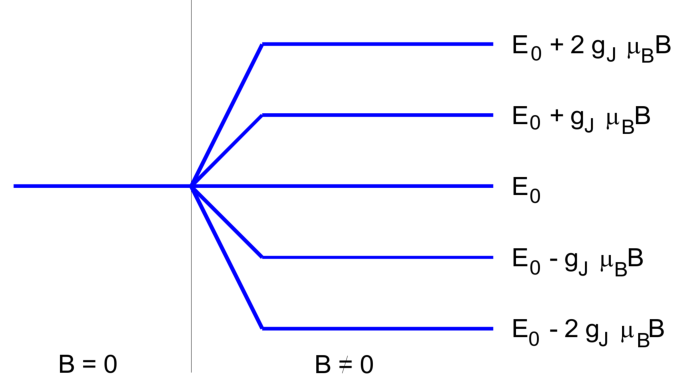
\includegraphics[width=0.8\textwidth]{images/V27_1.pdf}
  \caption{Energieaufspaltung bei einem Gesamtdrehimpuls $J = \num{2}$ \cite{anleitung}.}
  \label{abb:aufspaltung}
\end{figure}

\subsection{Auswahlregeln}
\label{sec:Auswahlregeln}
Durch die sogennanten Auswahlregeln, wird beschrieben, welche Übergänge zwischen
Energieniveaus möglich sind und welche nicht. Dazu wird die zeitabhängige
Schrödinger-Gleichung
\begin{align}
  \left( -\frac{\hbar^2}{2m}\Delta+U-i\hbar \frac{\delta}{\delta t} \right)\Phi\left(\vec{r}, t \right) = 0
  \label{eqn:schroedinger}
\end{align}
durch den Ansatz ebener Wellen kann bei einem Strahlungsübergang zwischen \alpha
und \beta eine Linearkbination der Lösungen mit den Normierungsbedingungen $C_\alpha$
und $C_\beta$ gebildet werden.
\begin{align}
  \Phi_\text{ges} = C_\alpha \Phi_\alpha\left(\vec{r}\right)\exp{\left(-\frac{i}{\hbar}E_\alpha t\right)} + C_\beta \Phi_\beta\left(\vec{r}\right)\exp{\left(-\frac{i}{\hbar}E_\beta t\right)}
  \label{eqn:ebenewelle}
\end{align}
Im Weiteren wird mittels Poynting-Vektor der Emitierten Strahlung die Auswahlregel
\begin{align}
  \Delta m = 0, \pm 1
  \label{eqn:auswahl}
\end{align}
verwendet. Dabei bezieht sich $\Delta m$ auf die Differenz der Orientierungsquantenzahlen
$m_\alpha$ und $m_\beta$ . Wird diese Bedingung erfüllt, so wird zwischen $\Delta m = 0$
und $\Delta m = \pm 1$ unterschieden. Beim ersten Fall ist die Stralung linear zum
Magnetfeld polarisiert, während im zweiten Fall eine zirkulare Polarisation vorliegt.


\subsection{Normaler-/Anormaler Zeemann-Effekt}
\label{sec:Zeemann}
Bei ausgeschaltetem Magnetfeld und Vernachlässigung des Spins ($S = \num{0}$) wird
der Effekt der Aufspaltung von Spektrallinien normaler Zeemann-Effekt genannt.
Ein Beispiel für die Aufspaltung der Energieniveaus mit $J = 1$ ist in Abbildung
\ref{abb:normal} zu sehen. Nach Formel \ref{eqn:lande} folgt, dass die Aufspaltungen
unabhängig von den Quantnzahlen sind und damit für alle Gesamtdrehimpulse $\text{g}_\text{J} = 1$
gilt. Daraus folgt, dass die zuvor aufgespaltenen Energieniveaus äquidistant sind.
\begin{figure}[htb]
  \centering
  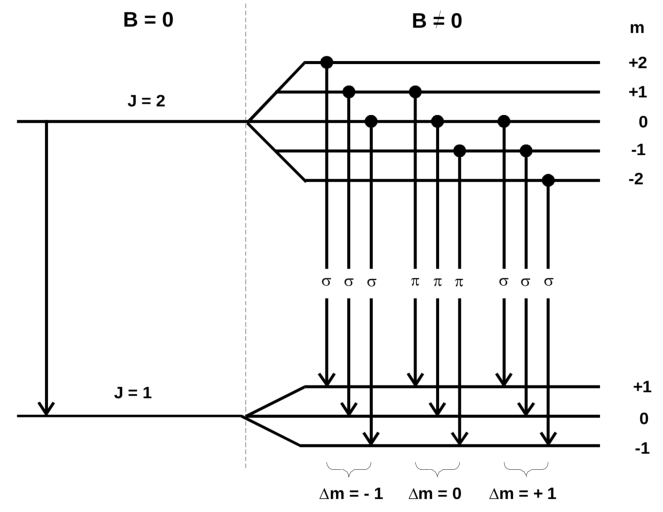
\includegraphics[width=0.8\textwidth]{images/V27_3.pdf}
  \caption{Linienaufspaltung der Spektrallinien beim normalen Zeemann-Effekt
  \cite{anleitung}.pdf.}
  \label{abb:normal}
\end{figure}
In Abbildung \ref{abb:normal} sind die Auswahlregeln den Linien der Aufspaltung
zugeordnet.
Dabei sind Aufspaltungslinien mit $\Delta m = \num{0}$, sog. \pi-Linien, nur in
einer Beobachtungsrichtung senkrecht zu den Feldlinien des Magnetfeldes liegt.
Gilt im anderen Fall $\Delta m = \pm 1$, so sind die Linien bei transversaler
Beobachtung linear polarisiert. Diese Beziehung der Beobachtungsweisen, sind
in Abbildung \ref{abb:spektral} zu erkennen.
\begin{figure}[htb]
  \centering
  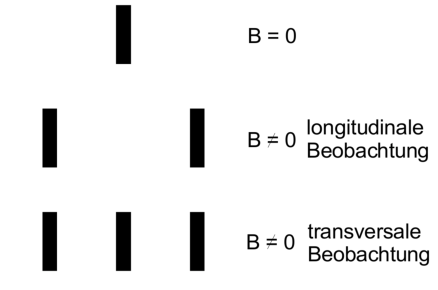
\includegraphics[width=0.8\textwidth]{images/V27_4.pdf}
  \caption{Spektrallinienaufspaltung beim normalen Zeemann-Effekt \cite{anleitung}.}
  \label{abb:spektral}
\end{figure}

Im Falle des Anormalen Zeemann-Effektes wird der Spin mit in Betracht gezogen, es
gilt also ($S \neq \num{0}$). Hier wird nicht die zeitabhängige Schrödingergleichung,
sondern die Dirac-Gleichung betrachtet. Es folgt, dass auch in diesem Fall, die
zuvor erwähnten Auswahlregeln noch gültig sind.
bei einem Übergang zwischen den Spektrallinien wird durch Hinzunahme der Quantenzahlen
der beiden Übergangsniveaus $L_1, S_1, J_1$ sowie $L_2, S_2, J_2$  die Energie
\begin{align}
  E = \left(m_1 g(L_1, S_1, J_1) - m_2 g(L_2, S_2, J_2) \right)\mu_\text{B} B + E_0
\end{align}
emittert. $E_0$ beschreibt hier die Energie ohne angelegtes Magnetfeld ($\vec{B} = \num{0}$).
Durch die Hinzunahme der Quantenzahlen $L, S$ und $J$ weren mehr Aufspaltungslinien
sichtbar. Dies ist in Abbildung \ref{abb:anormal} aufgezeichnet.
\begin{figure}[htb]
  \centering
  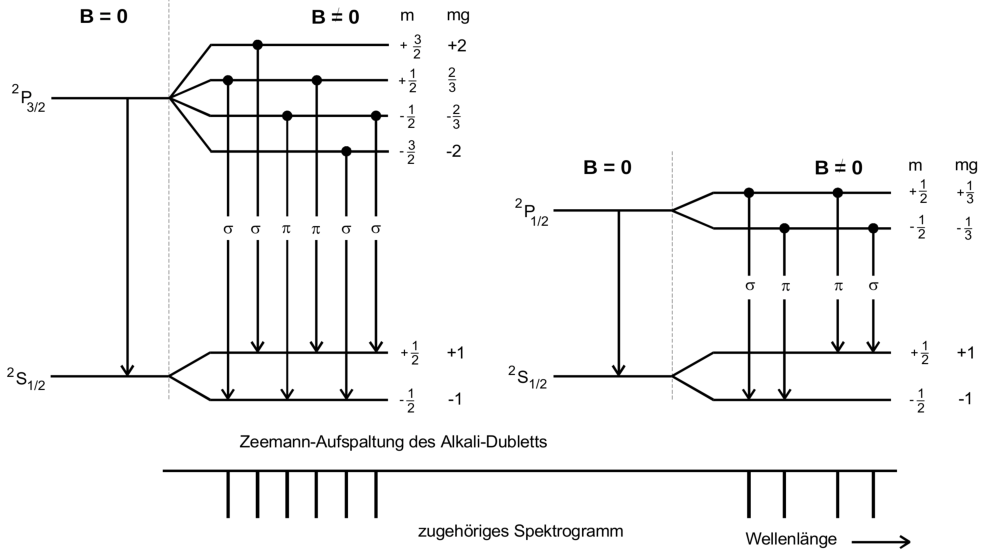
\includegraphics[width=0.8\textwidth]{images/V27_5.pdf}
  \caption{Linienaufspaltung der Spektrallinien beim annormalen Zeemann-Effekt
  am Beispiel eines Alkali-Dubletts \cite{anleitung}.}
  \label{abb:anormal}
\end{figure}
